\documentclass{article}
\usepackage{bookmark}

% Language setting
\usepackage[T1]{fontenc}
\usepackage[french]{babel}

% Set page size and margins
\usepackage[letterpaper,top=2cm,bottom=2cm,left=3cm,right=3cm,marginparwidth=1.75cm]{geometry}
\usepackage{float}
% Useful packages
\usepackage{amsmath}
\usepackage{graphicx}
\usepackage[colorlinks=true, allcolors=blue]{hyperref}


\title{Rapport d'Analyse SonarQube}
\author{Adil ABBADI \and Abdelhak MEKAOUI}
\date{}
\begin{document}
\maketitle

\begin{abstract}
Ce rapport présente les résultats de l'analyse de code effectuée avec SonarQube sur un projet Spring Boot pour la gestion des formations e-learning.
\end{abstract}

\section{Introduction}

Ce document décrit l'utilisation de SonarQube pour analyser un projet Spring Boot dédié à la gestion des formations e-learning. SonarQube est un outil puissant pour l'inspection continue de la qualité du code, permettant de détecter les bugs, les vulnérabilités et les mauvaises pratiques.

\section{Contexte et Objectifs}

Dans le cadre de ce module, on est chargé d’évaluer et d’améliorer la qualité d’un projet Spring Boot développé lors d’un précédent cycle. Le projet comporte une analyse approfondie du code source à l'aide de SonarQube, des tests logiciels (boîte blanche, boîte noire, et performance), ainsi que l’intégration d’outils et de méthodologies modernes de qualité logicielle. L’objectif est de détecter, analyser, et corriger les erreurs, tout en mettant en place des solutions d’amélioration continue basées sur les principes DevOps.

\section{Résultats Attendus}

\subsection{Contexte du projet}

\begin{enumerate}
    \item Présentation du projet logiciel. \\
    Le projet consiste en une application web de gestion des formations e-learning, permettant aux utilisateurs de s’inscrire, de suivre des cours, et de passer des évaluations en ligne.
    \begin{figure}[H]
    \centering
    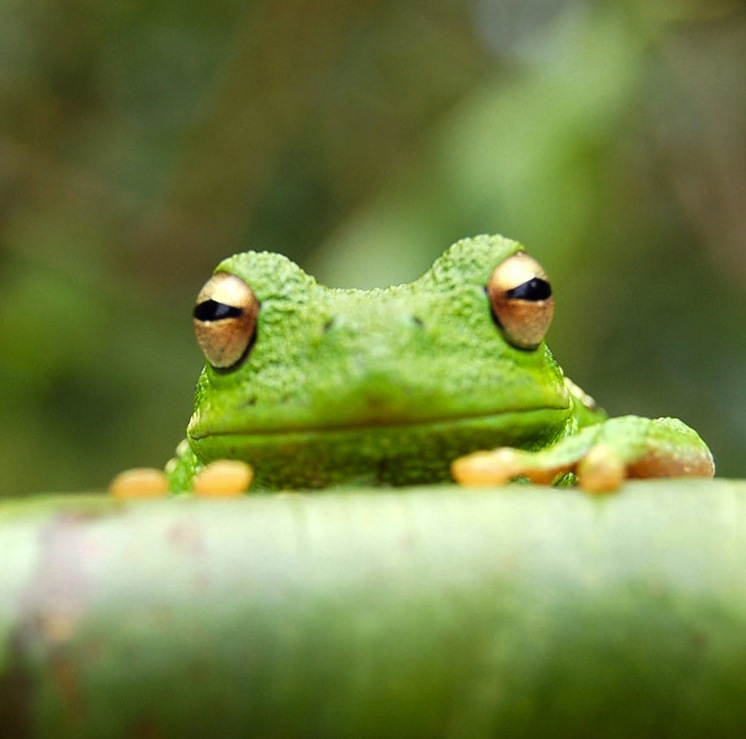
\includegraphics[width=0.5\linewidth]{assets/frog.jpg}
    \caption{\label{fig:frog}Interface utilisateur du logiciel .}
    \end{figure}

    \item Les erreurs rencontrées. \\
    Durant le développement et l'utilisation de l'application, plusieurs erreurs ont été identifiées, notamment des bugs fonctionnels, des problèmes de performance, et des vulnérabilités de sécurité.

    \item Les méthodes employées pour détecter les erreurs. \\
    Pour détecter les erreurs, diverses méthodes ont été utilisées, telles que les tests manuels, les tests automatisés, les revues de code, et l'analyse statique du code avec des outils comme SonarQube.
 
\end{enumerate}

\subsection{Analyse de la qualité avec SonarQube}

\begin{enumerate}
    \item Installer ou configurer un serveur SonarQube localement ou en ligne.
    \begin{figure}[H]
        \centering
        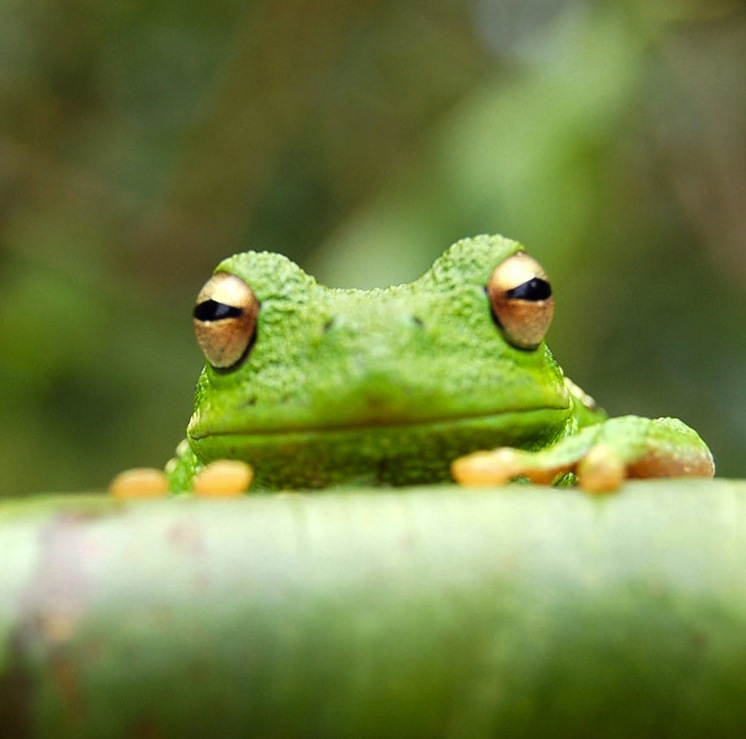
\includegraphics[width=0.5\linewidth]{assets/frog.jpg}
        \end{figure}
    \item Importer le code source du projet précédent dans SonarQube .
    \begin{figure}[H]
        \centering
        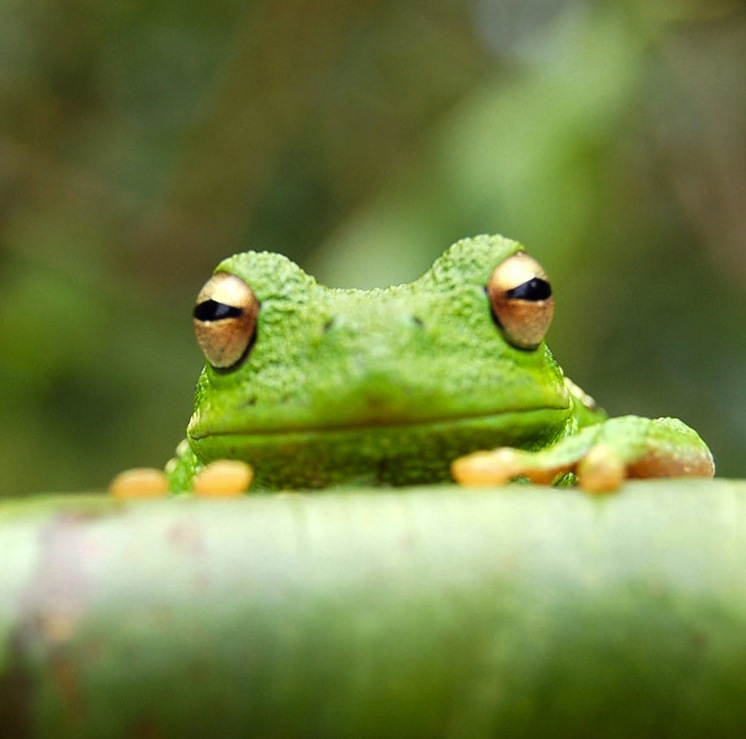
\includegraphics[width=0.5\linewidth]{assets/frog.jpg}
        \end{figure}
    
    \item Examiner les métriques générées par SonarQube.
    \begin{figure}[H]
        \centering
        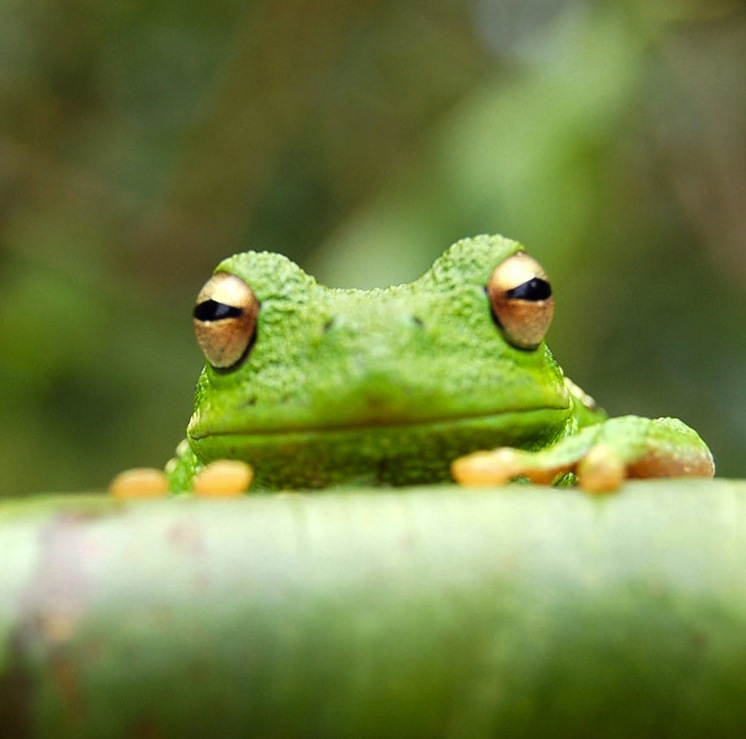
\includegraphics[width=0.5\linewidth]{assets/frog.jpg}
        \end{figure}
    \item Identifier les points faibles et proposer des améliorations.
    \begin{figure}[H]
        \centering
        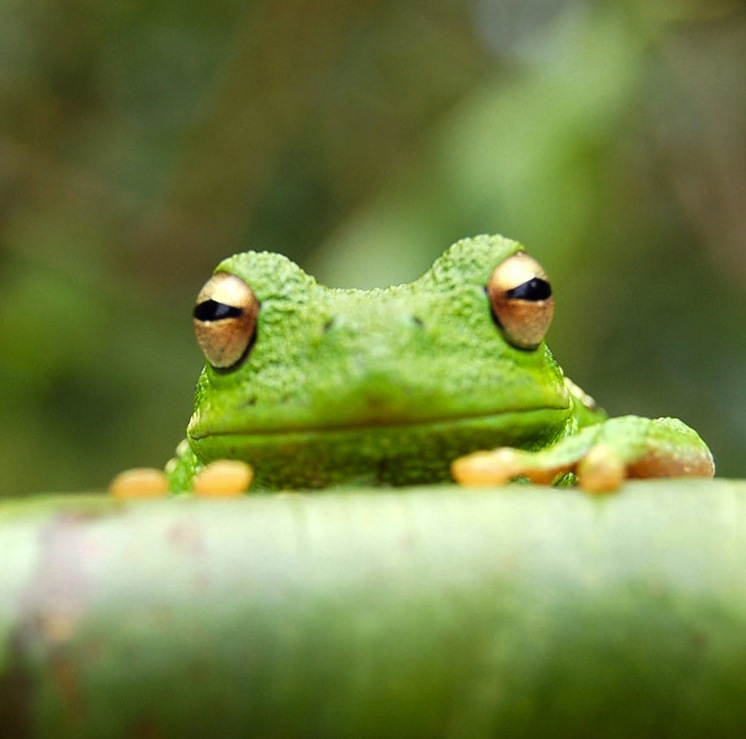
\includegraphics[width=0.5\linewidth]{assets/frog.jpg}
        \end{figure}
\end{enumerate}

\subsection{Tests Boîte Blanche}

\begin{enumerate}
    \item Les tests unitaires.
    \begin{figure}[H]
        \centering
        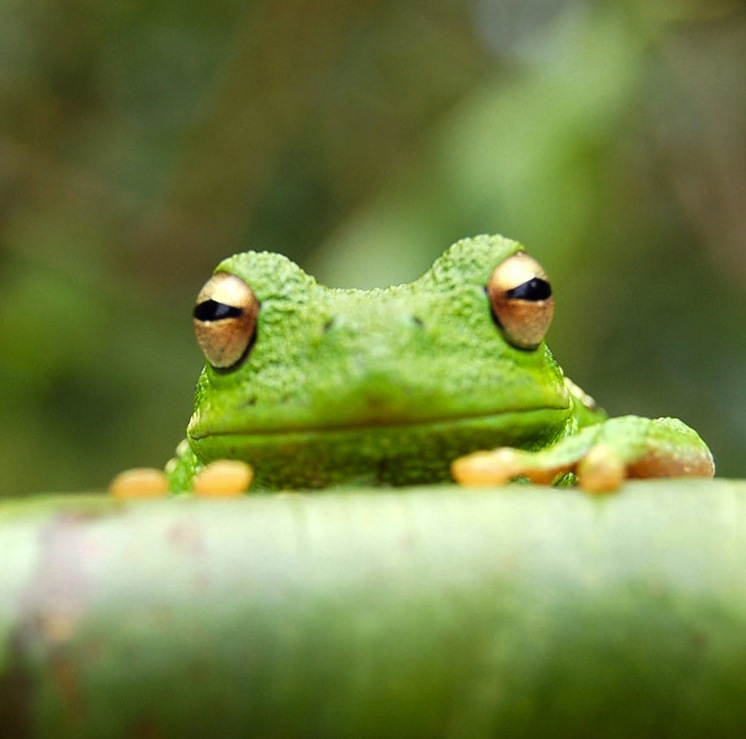
\includegraphics[width=0.5\linewidth]{assets/frog.jpg}
        \end{figure}

    \item Réévaluer la couverture de code avec SonarQube après chaque itération des tests.
    \begin{figure}[H]
        \centering
        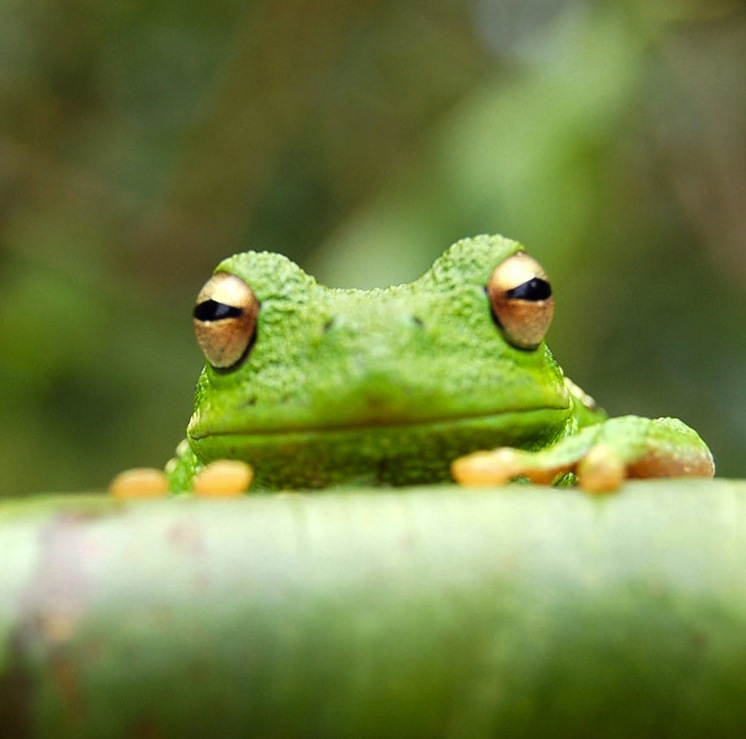
\includegraphics[width=0.5\linewidth]{assets/frog.jpg}
        \end{figure}




    \item Documenter l’efficacité des tests en mettant en avant les erreurs détectées et corrigées.
    \begin{figure}[H]
        \centering
        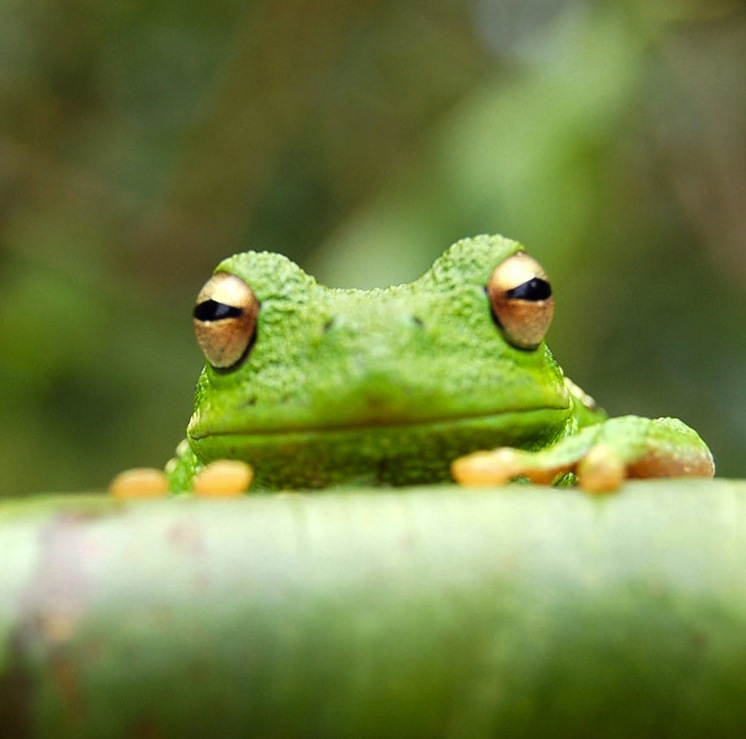
\includegraphics[width=0.5\linewidth]{assets/frog.jpg}
        \end{figure}

\end{enumerate}

\subsection{Tests Boîte Noire}

\begin{enumerate}
    \item Utilisation de selenium pour simuler utilisation de application.
    \begin{figure}[H]
        \centering
        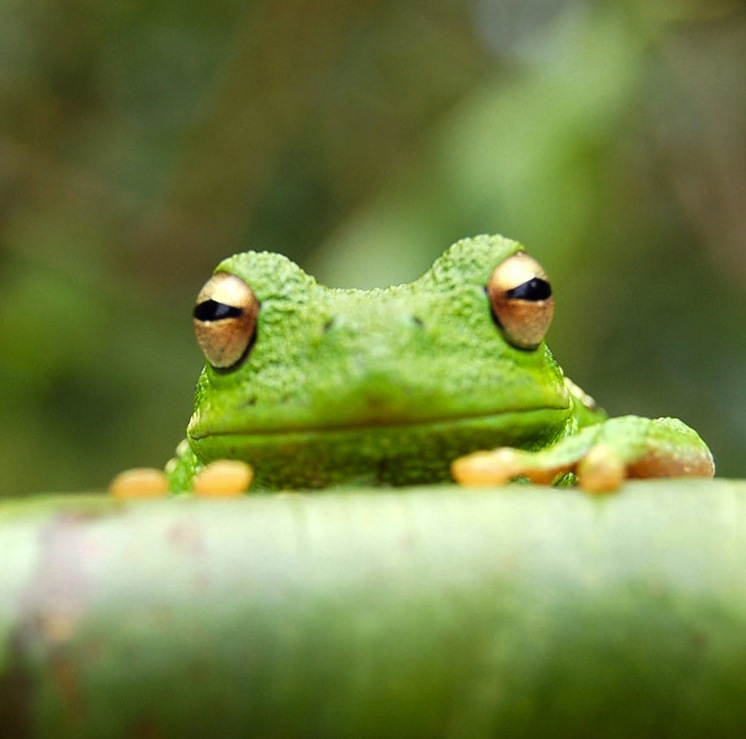
\includegraphics[width=0.5\linewidth]{assets/frog.jpg}
        \end{figure}
    \item Tester les principales fonctionnalités de l’application en suivant différents cas d’utilisation.
    \begin{figure}[H]
        \centering
        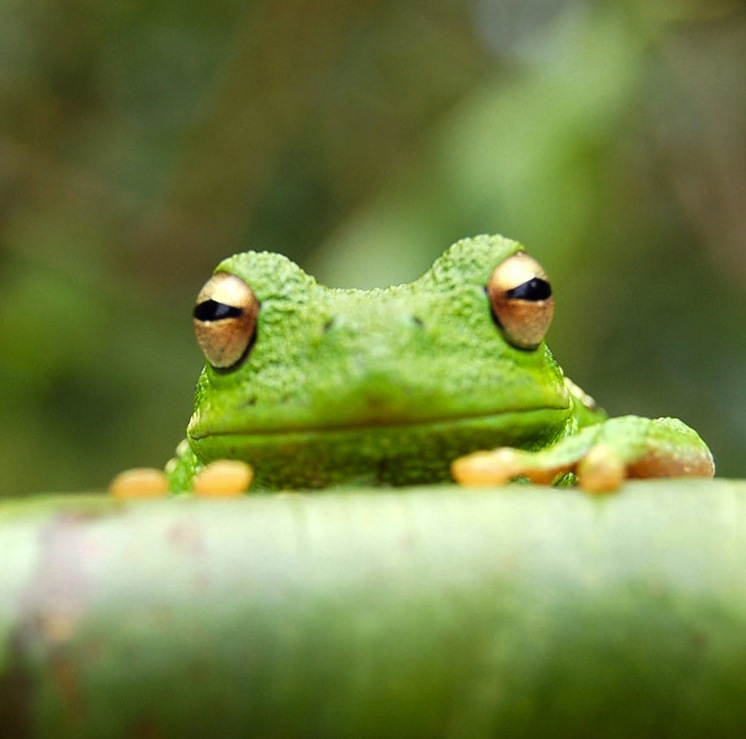
\includegraphics[width=0.5\linewidth]{assets/frog.jpg}
        \end{figure}
\end{enumerate}

\subsection{Tests de Performance}

\begin{enumerate}
    \item Test de performance tel que JMeter.
    \begin{figure}[H]
        \centering
        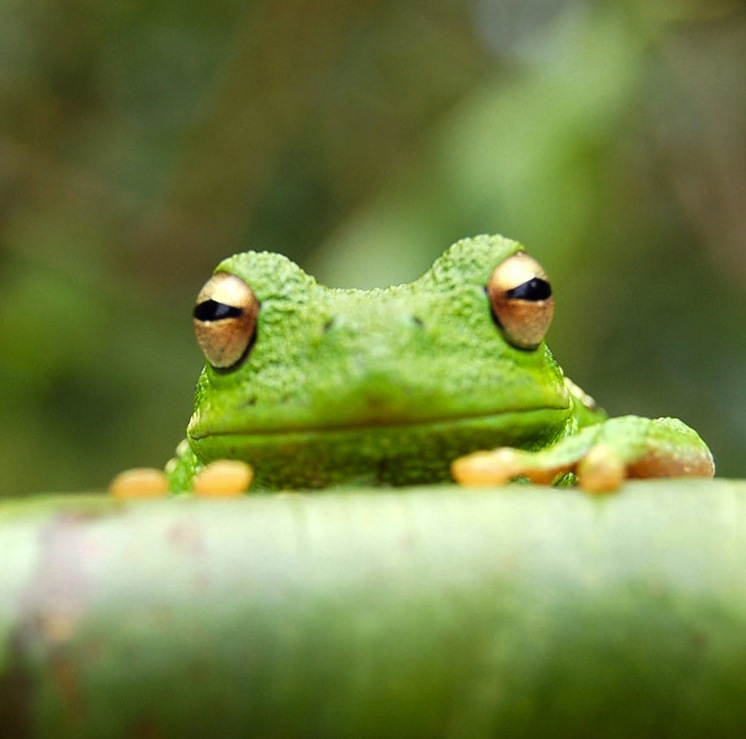
\includegraphics[width=0.5\linewidth]{assets/frog.jpg}
        \end{figure}
    \item Test de stress en simulant 500 utilisateurs.
    \begin{figure}[H]
        \centering
        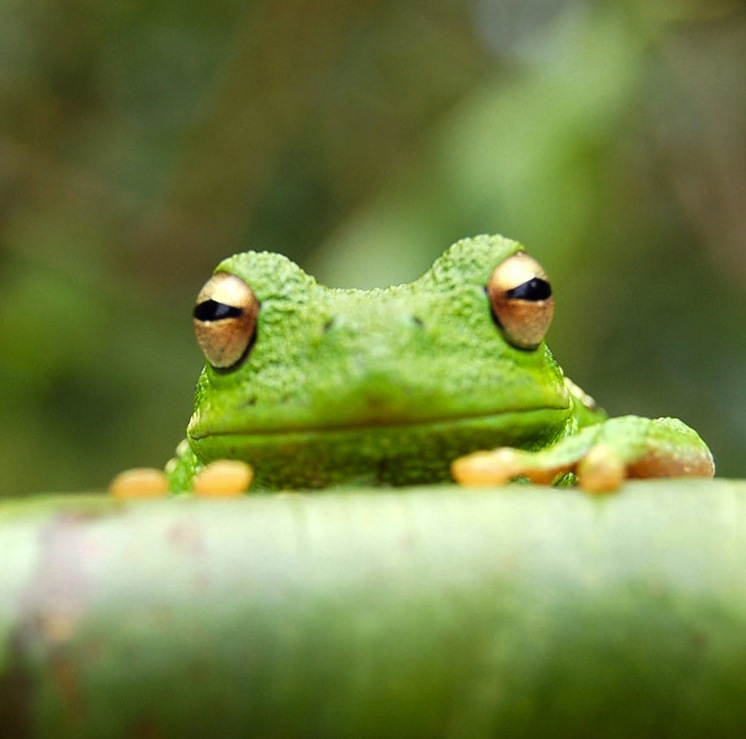
\includegraphics[width=0.5\linewidth]{assets/frog.jpg}
        \end{figure}
    \item Test de charge, en doublant puis en triplant le nombre maximal d’utilisateurs.
    \begin{figure}[H]
        \centering
        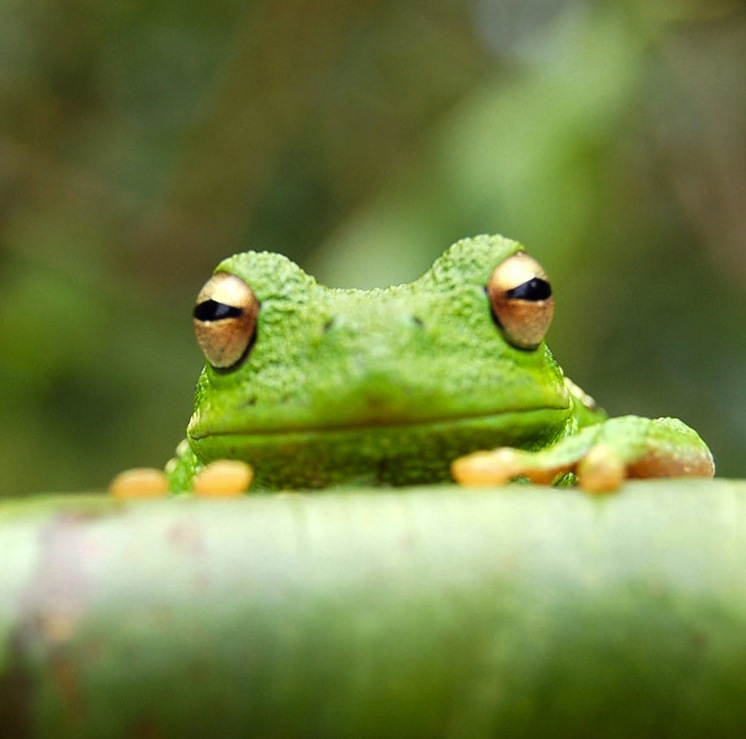
\includegraphics[width=0.5\linewidth]{assets/frog.jpg}
        \end{figure}
\end{enumerate}

\subsection{Intégration DevOps et Automatisation des Tests}

\begin{enumerate}
    \item CI/CD en utilisant Jenkins .
    \begin{figure}[H]
        \centering
        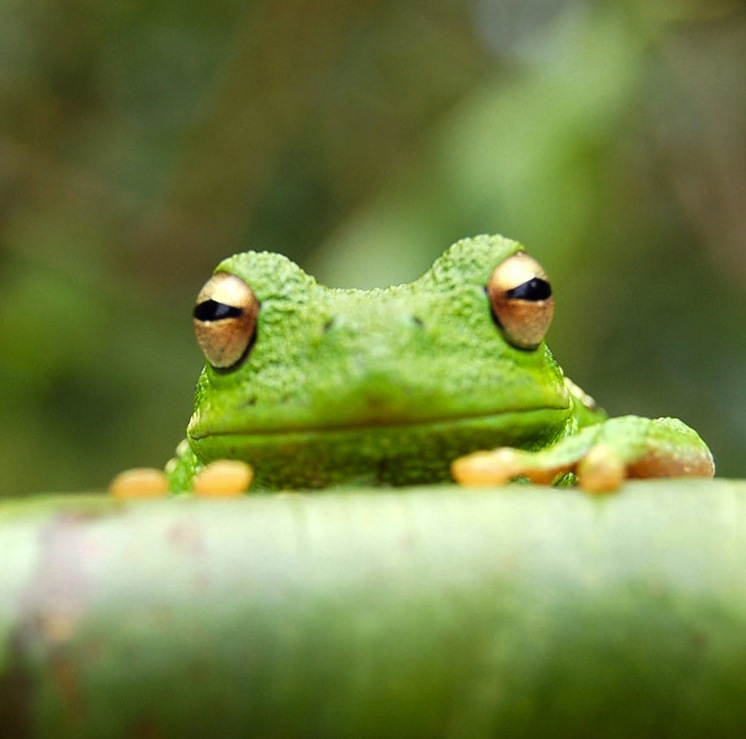
\includegraphics[width=0.5\linewidth]{assets/frog.jpg}
        \end{figure}
    \item Configurer des alertes pour signaler les échecs de tests.
    \begin{figure}[H]
        \centering
        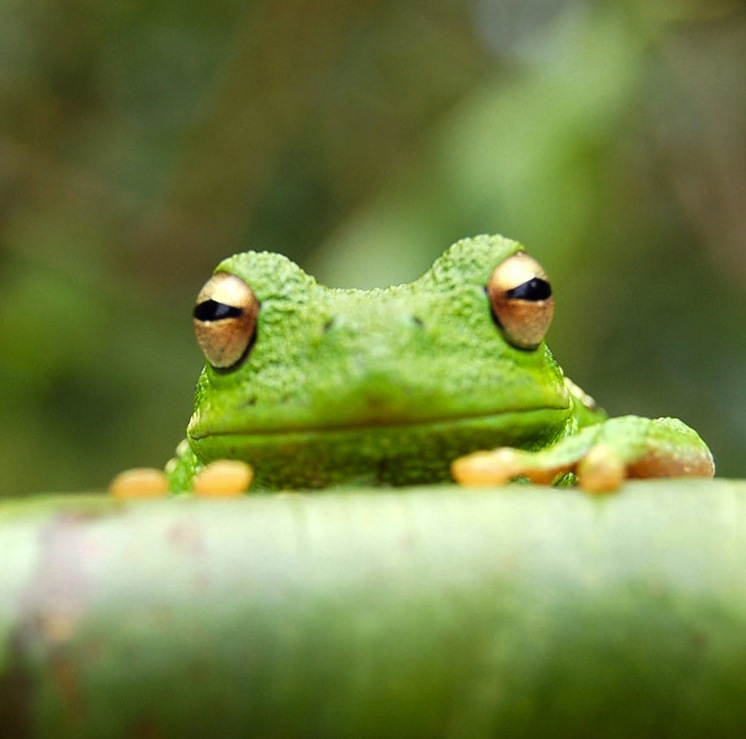
\includegraphics[width=0.5\linewidth]{assets/frog.jpg}
        \end{figure}
    \item Automatiser le déploiement continu des versions en utilisant webhook.
    \begin{figure}[H]
        \centering
        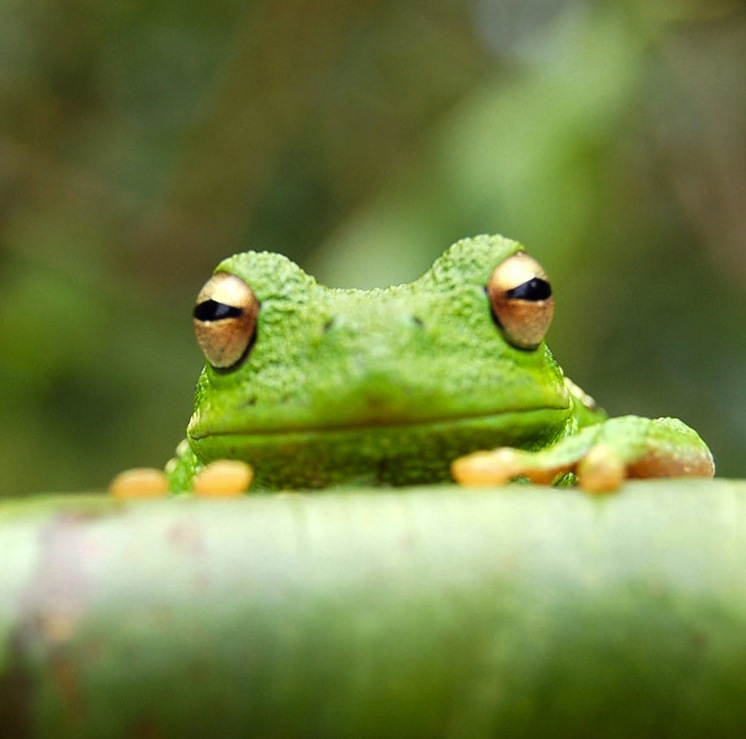
\includegraphics[width=0.5\linewidth]{assets/frog.jpg}
        \end{figure}
\end{enumerate}


\section{Résultats de l'Analyse}

Les résultats de l'analyse SonarQube sont présentés ci-dessous. Ils incluent des métriques sur la qualité du code, les bugs détectés, les vulnérabilités et les duplications de code.


\subsection{Qualité du Code}

\begin{figure}[H]
    \centering
    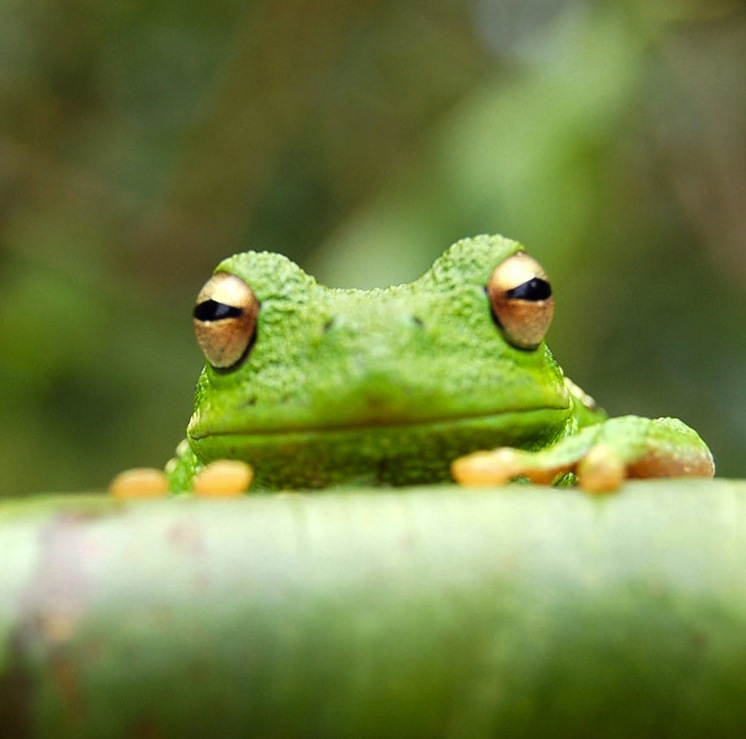
\includegraphics[width=0.5\linewidth]{assets/frog.jpg}
    \end{figure}

\subsection{Bugs et Vulnérabilités}

\begin{figure}[H]
    \centering
    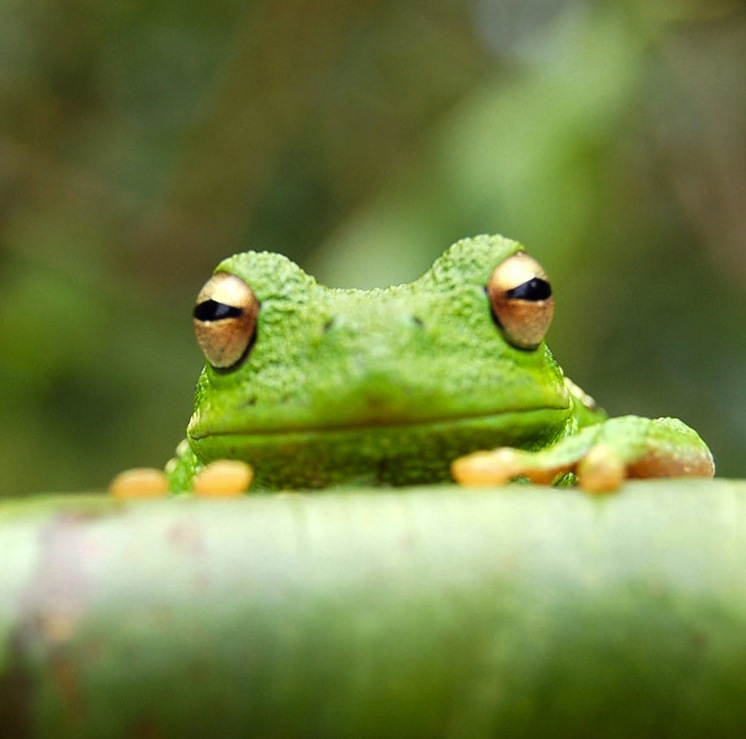
\includegraphics[width=0.5\linewidth]{assets/frog.jpg}
    \end{figure}

\subsection{Duplications de Code}

\begin{figure}[H]
    \centering
    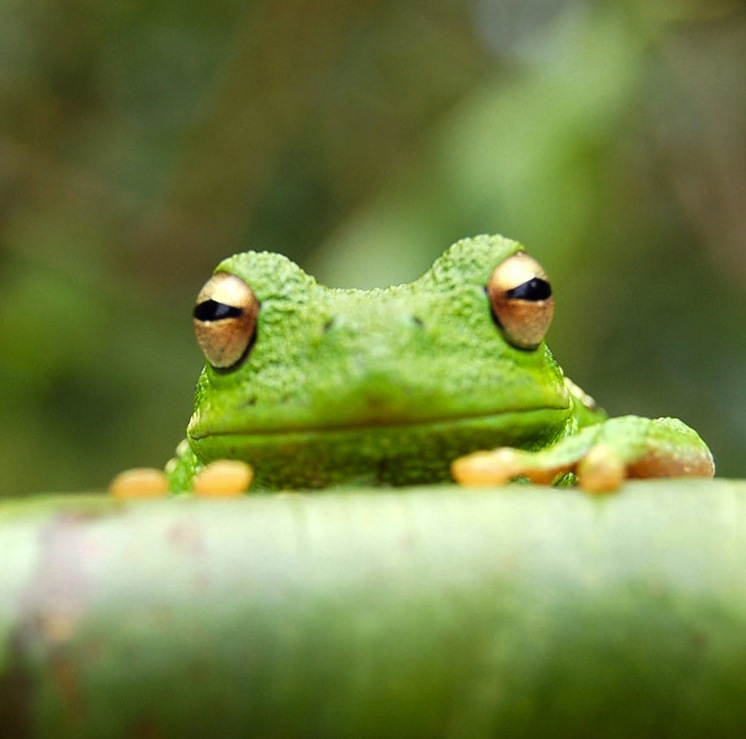
\includegraphics[width=0.5\linewidth]{assets/frog.jpg}
    \end{figure}

\section{Conclusion}

En conclusion, l'utilisation de SonarQube pour analyser le projet Spring Boot de gestion des formations e-learning a permis d'identifier plusieurs aspects à améliorer en termes de qualité du code, de sécurité et de maintenabilité. Les résultats obtenus fournissent une base solide pour des améliorations futures.


% \cite{some_reference}




\end{document}